\subsubsection{Vorteile von Polycarbonat gegenüber anderen Materialien}

Polycarbonat wurde 1953 von dem bei der Firma Bayer angestellten Chemiker
Hermann Schnell entdeckt. Der neue Kunststoff wurde später unter dem Namen
Makrolon\textsuperscript{\textregistered} vermarktet. \cite{cuzpc}

Nachdem Philips seinen ersten CD-Prototypen hergestellt hatte, suchte man nach
einem Trägermaterial, welches für die Massenproduktion mittels
Spritzgussverfahren geeignet ist. Hierfür ist Polycarbonat nahezu perfekt. Die
niedrige Viskosität ermöglicht eine fehlerfreie Übertragung der Pitstruktur von
der Matrize auf die Polycarbonatscheibe. Hohe Transparenz und ein konstanter
Brechungsindex\footnote{Verhältnis der Lichtgeschwindigkeit und der
Ausbreitungsgeschwindigkeit von Licht im untersuchten Material} erlauben ein
unabgeschwächtes Durchdringen des Laserstrahls durch das Trägermaterial. Eine
hohe Erweichungstemperatur bei ca. 149°C\cite{cuzpc2} und Resistenz gegenüber
physikalischen Belastungen machen Polycarbonat ebenfalls alltagstauglich.
\cite{cfcd}

\autoref{fig:cdpcpmma} vergleicht Polycarbonat (PC) und Polymethylmethacrylat
(PMMA) in Bezug auf Eigenschaften, die für die Herstellung und Benutzung der CD
relevant sind. Die Eignung nimmt in den jeweiligen Punkten von innen nach außen
zu. PMMA schneidet in fast allen Punkten mit Bestnoten ab. Polymethylmethacrylat
ist jedoch in den Kategorien Wärmeformbeständigkeit und Wasseraufnahme PC
unterlegen. Dies sowie das gute Abschneiden bei den anderen Eigenschaften macht
Polycarbonat zum bevorzugten Kunststoff für die CD-Produktion.

\begin{figure}[h]
    \begin{center}
        \begin{minipage}[t]{\textwidth}
            \begin{center}
                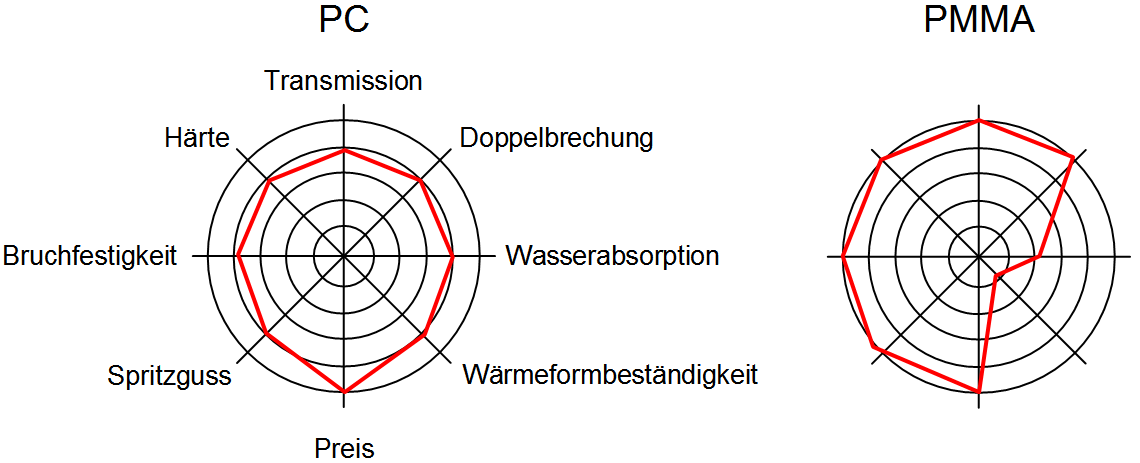
\includegraphics[height=0.1\textheight]{Bilder/Optische_Datentraeger_Die_Compact_Disc/Material_Polycarbonat/cdpcpmma.png}
                \caption[Vergleich zwischen PC und PMMA \newline Roth, Klaus: CD, DVD \& Co.: Die Chemie der schillernden Scheiben, in: Chemie in unserer Zeit (41/2007), S. 337]{Vergleich zwischen PC und PMMA}
                \label{fig:cdpcpmma}
            \end{center}
        \end{minipage}
    \end{center}
\end{figure}
